\documentclass[../main.tex]{subfiles}

\begin{document}

\chapter{Benchmark Comparison}

We now have a data-driven methodology for deriving learned sector universes (addressing RG-1), and have developed a objetive criteria-driven ranking methodology to compare the learned sector universes against each other, addressing RG-2. The final step is to evaluate our risk-adjusted return optimal learned sector universe against the benchmark classification. Thus, this section addresses the third and final research goal, RG-3 (see Section~\ref{research_goals:specific_research_goals}).

\begin{table}[h!]
    \centering
    \begin{tabular}{| c | c |}
        \hline
        &  \\
        RG-3 & Evaluate our risk-adjusted return optimal sector universe against the benchmark. \\
        & \\
        \hline
    \end{tabular}
\end{table}

% TEMPORARY


Analyzing each of the new learned sectors in turn, it is clear that beyond the large sectors \textit{Alpha} and \textit{Golf}, a large majority of the remaining sectors are extremely small with respect to their numbers of component assets. Despite this however, the two large (major) sectors - as well as a selection of the smaller (i.e. minor) sectors - have an extremely high dispersion rate relative to the benchmark. That is, there doesn't seem to be a high level of congruence between the old and new sector assignments.

Both major learned sectors \textit{Alpha} and \textit{Golf} retain a large number of assets as their components. Particularly, it can be observed that learned sector \text{Alpha} contains a majority of the benchmark \textit{Financials} sector, and the benchmark \textit{Utilities} sector. Given that these sector assignments are derived from fundamentals data, this is a particularly interesting result, as both \textit{Financials} and \textit{Utilities} have become extremely risk-averse businesses over the last decade; \textit{Financials} due to the Great Recession of 2008, and \textit{Utilities} due to extensive capital damange incurred by the increased severity and number of Natural Disasters. This grouping indicates that the capital structure of these businesses are also becoming increasingly similar.

Considering learned sector \textit{Golf}, it seems to be a mini-index within the oringal sector universe. From a component count perspective, it ingests a large amount of the benchmark \textit{Consumer Discretionary} and \textit{Consumer Staples} industries, as well as large swaths of industries that form the backbone of the US Economy as a whole; namely, the \textit{Information Techonology}, \textit{Industrials}, and \textit{Real Estate} sectors.
% END TEMP

In this chapter we make comparison between our optimal sector universe of maximum Sharpe Ratio and benchmark sector universe. We compare each of the performance metric of both sector universes and demonstrate which sector universe has better risk-adjusted return.  

\section{Comparison Analysis}

Our benchmark sector universe is GICS S\&P 500 sectors universe. We do the backtesting of benchmark sector universe and calculate the same index we talk about in above chapters, which are cumulative ETF restructuring turnover, cumulative portfolio rebalancing turnover, portfolio return and portfolio Sharpe Ratio  respectively. The graphs of comparison between benckmark sector universe and our optimal sector unverse are: 

\begin{figure}[H]
    \centering
    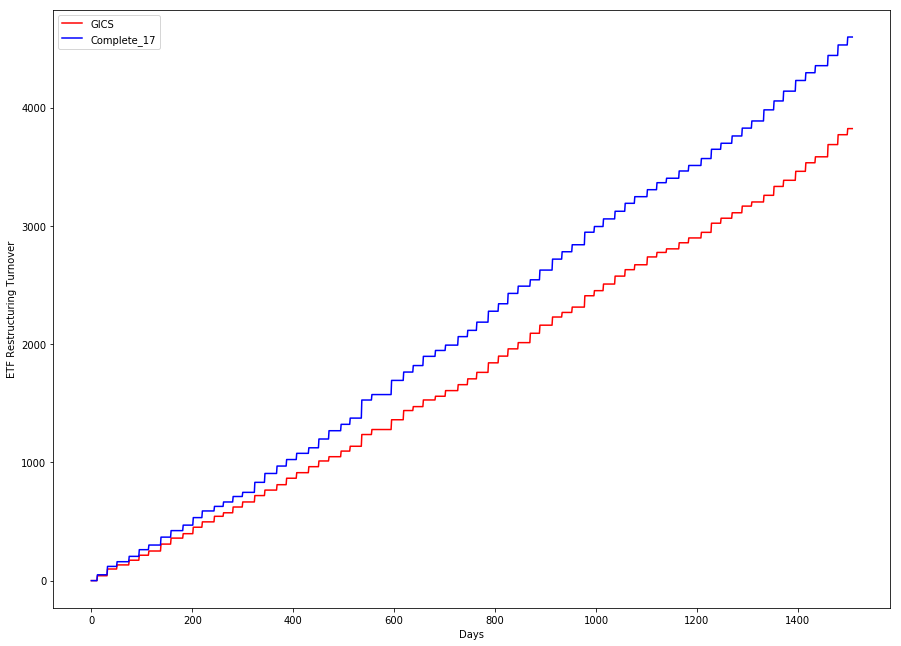
\includegraphics[scale=0.4]{images/etf_restrut_compare.png}
    \caption{Cumulative ETF Restructuring Turnover Comparison}
    \label{fig:benchmark_comparison:restrut_turnover_comparison}
\end{figure} 

\begin{figure}[H]
    \centering
    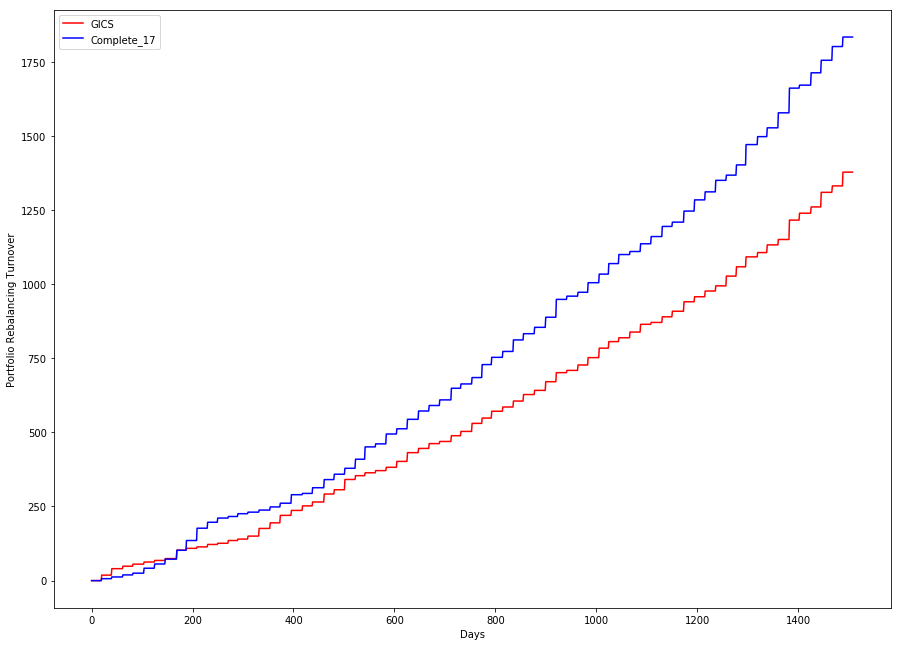
\includegraphics[scale=0.4]{images/port_rebal_compare.png}
    \caption{Cumulative Portfolio Rebalancing Turnover Comparison}
    \label{fig:benchmark_comparison:rebal_turnover_comparison}
\end{figure}

\begin{figure}[H]
    \centering
    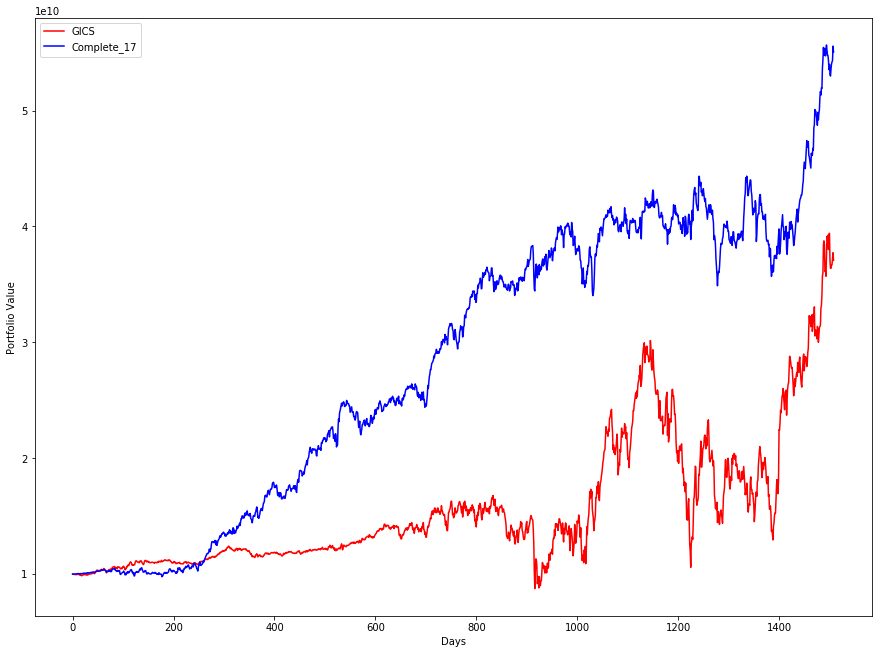
\includegraphics[scale=0.4]{images/value_compare.png}
    \caption{Portfolio Return Comparison}
    \label{fig:benchmark_comparison:retuern_comparison}
\end{figure}

 \begin{figure}[H]
    \centering
    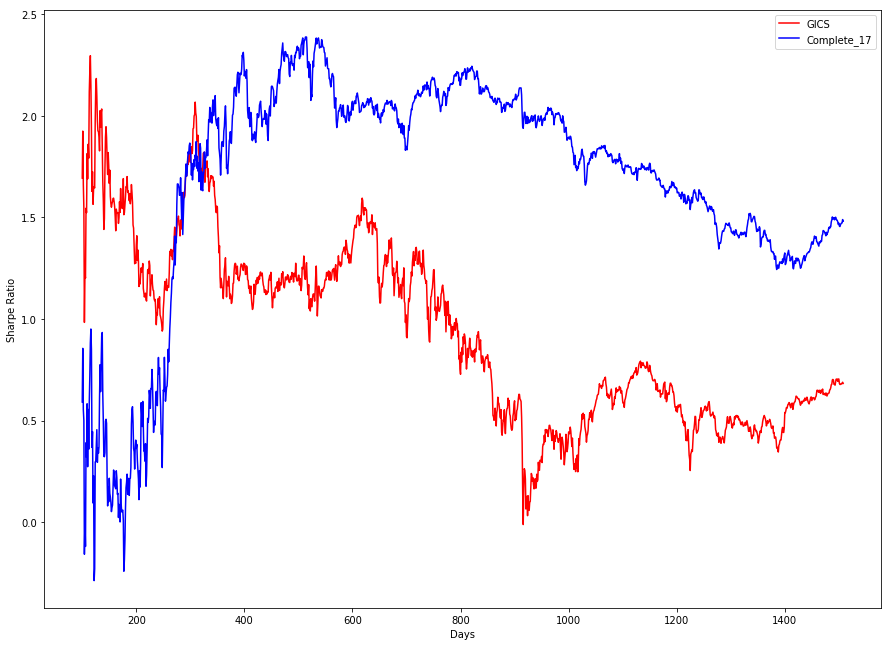
\includegraphics[scale=0.4]{images/sharpe_compare.png}
    \caption{Portfolio Sharpe Ratio Comparison}
    \label{fig:benchmark_comparison:sharpe_comparison}
\end{figure}

All red curves represent performances of benchmark sector universe and all blue curves represent performance optimal sector universe with Complete Linkage,16 Sectors. The graphs show that for cummulative turnovers,benchmark sector universe perform better than our optimal universe. One possible reason is the structure of our optimal sector. We will explore the relationship of sector structure and turnover in future work. 

Back to the topic, we highlight the comparison of Sharpe Ratio since it reflect the risk-adjusted return. From the graph, it is clear that the Sharpe Ratio of our optimal sector universe is higher than that of benchmark sector universe for most of the time during backtesting period. This indicates that our sector universe from machine-learning algorithm has hagher risk-adjusted return rhan benchmark. 

\end{document}